\subsection{Supervised and unsupervised learning}
Derived from the different kinds of tabular data, we have two fundamental learning paradigms. Exemplary input data and possible results for both paradigms can be seen in \ref{fig:1_sv_vs_usv}.

\begin{figure}[h]
  \centering
  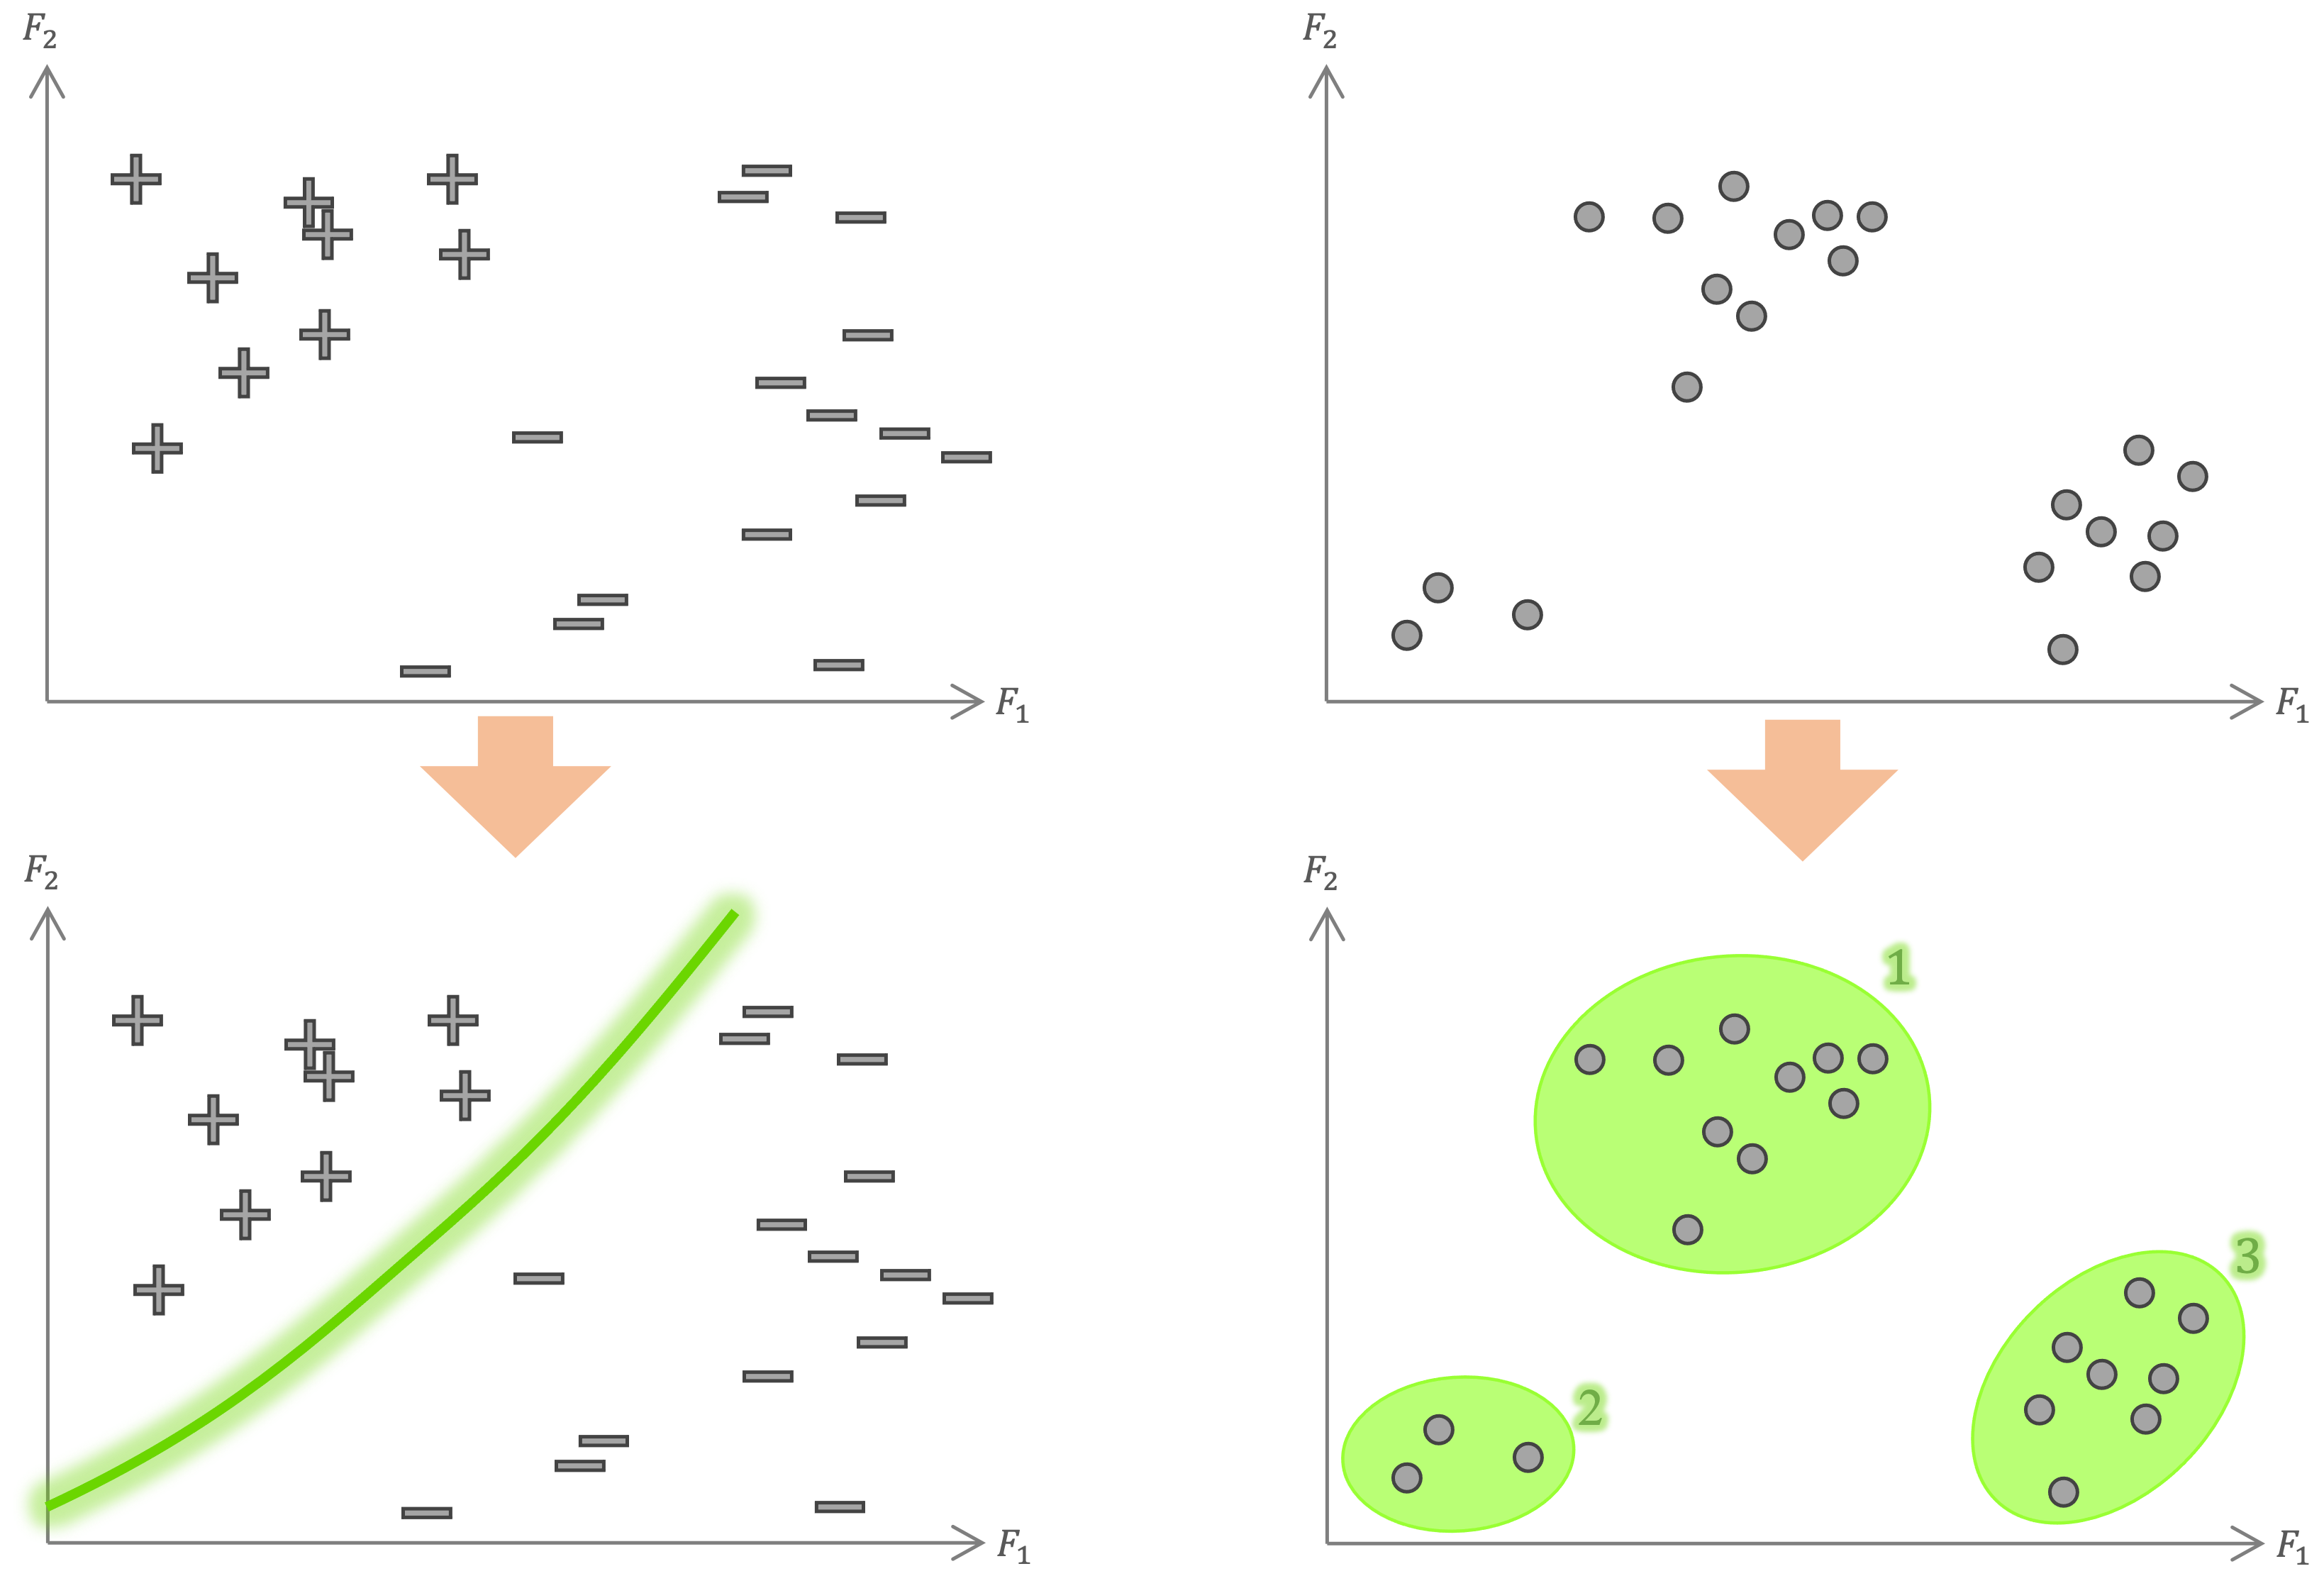
\includegraphics[width=0.7\textwidth]{assets/basics/SV_vs_US.png}
  \caption{Comparing supervised (left) and unsupervised (right) learning}
  \label{fig:1_sv_vs_usv}
\end{figure}

In the case of labeled data, we can apply \textbf{supervised learning}\sidenote{Supervised learning}. The goal is to find a "rule" in terms of descriptive features explaining the target feature as well as possible. Examples include:
\begin{itemize}
  \item Hospital environments where:
  \begin{itemize}
    \item The target variable can be {\color{ForestGreen}recover (yes or no)}, and 
    \item The descriptive variables can be {\color{ForestGreen}age, gender, smoking, $\dots$}
  \end{itemize}
  \item University environments where:
  \begin{itemize}
    \item The target variable can be {\color{ForestGreen}drops out (yes or no)}, and 
    \item The descriptive variables can be {\color{ForestGreen}mentor, prior education, $\dots$}
  \end{itemize}
  \item Production environments where:
  \begin{itemize}
    \item The target variable can be {\color{ForestGreen}order is delivered in time (yes or no)}, and 
    \item The descriptive variables can be {\color{ForestGreen}product, agent, $\dots$}
  \end{itemize}
\end{itemize}

In contrast to labeled data, we can also have instances without target labels, where we can only apply techniques of \textbf{unsupervised learning}\sidenote{Unsupervised learning}. The goal is to find clusters or patterns.
\begin{itemize}
  \item \textbf{Clusters}\sidenote{Cluster} are homogeneous sets of instances. Examples include finding similar groups of patients, students, customers, orders, cars, companies, and so on.
  \item \textbf{Patterns}\sidenote{Pattern} on the other hand reveal hidden structures in the data, so basically the unknown unknowns. Rules of some form can be found in many environments and can for example look like this:
  \begin{itemize}
    \item Customers who buy bread and butter typically pay by phone.
    \item Patients who drink and smoke typically pay the hospital bill earlier than others.
    \item Products produced by team A on Monday tend to be returned more frequently by customers.
  \end{itemize} 
\end{itemize}

Interesting to regard is process discovery as a form of unsupervised learning in the way that a process model is just a very sophisticated rule. Important to mention, that this task can get very complex very quickly.
